% Options for packages loaded elsewhere
\PassOptionsToPackage{unicode}{hyperref}
\PassOptionsToPackage{hyphens}{url}
%
\documentclass[
  man,floatsintext]{apa6}
\usepackage{amsmath,amssymb}
\usepackage{lmodern}
\usepackage{iftex}
\ifPDFTeX
  \usepackage[T1]{fontenc}
  \usepackage[utf8]{inputenc}
  \usepackage{textcomp} % provide euro and other symbols
\else % if luatex or xetex
  \usepackage{unicode-math}
  \defaultfontfeatures{Scale=MatchLowercase}
  \defaultfontfeatures[\rmfamily]{Ligatures=TeX,Scale=1}
\fi
% Use upquote if available, for straight quotes in verbatim environments
\IfFileExists{upquote.sty}{\usepackage{upquote}}{}
\IfFileExists{microtype.sty}{% use microtype if available
  \usepackage[]{microtype}
  \UseMicrotypeSet[protrusion]{basicmath} % disable protrusion for tt fonts
}{}
\makeatletter
\@ifundefined{KOMAClassName}{% if non-KOMA class
  \IfFileExists{parskip.sty}{%
    \usepackage{parskip}
  }{% else
    \setlength{\parindent}{0pt}
    \setlength{\parskip}{6pt plus 2pt minus 1pt}}
}{% if KOMA class
  \KOMAoptions{parskip=half}}
\makeatother
\usepackage{xcolor}
\usepackage{graphicx}
\makeatletter
\def\maxwidth{\ifdim\Gin@nat@width>\linewidth\linewidth\else\Gin@nat@width\fi}
\def\maxheight{\ifdim\Gin@nat@height>\textheight\textheight\else\Gin@nat@height\fi}
\makeatother
% Scale images if necessary, so that they will not overflow the page
% margins by default, and it is still possible to overwrite the defaults
% using explicit options in \includegraphics[width, height, ...]{}
\setkeys{Gin}{width=\maxwidth,height=\maxheight,keepaspectratio}
% Set default figure placement to htbp
\makeatletter
\def\fps@figure{htbp}
\makeatother
\setlength{\emergencystretch}{3em} % prevent overfull lines
\providecommand{\tightlist}{%
  \setlength{\itemsep}{0pt}\setlength{\parskip}{0pt}}
\setcounter{secnumdepth}{-\maxdimen} % remove section numbering
% Make \paragraph and \subparagraph free-standing
\ifx\paragraph\undefined\else
  \let\oldparagraph\paragraph
  \renewcommand{\paragraph}[1]{\oldparagraph{#1}\mbox{}}
\fi
\ifx\subparagraph\undefined\else
  \let\oldsubparagraph\subparagraph
  \renewcommand{\subparagraph}[1]{\oldsubparagraph{#1}\mbox{}}
\fi
\newlength{\cslhangindent}
\setlength{\cslhangindent}{1.5em}
\newlength{\csllabelwidth}
\setlength{\csllabelwidth}{3em}
\newlength{\cslentryspacingunit} % times entry-spacing
\setlength{\cslentryspacingunit}{\parskip}
\newenvironment{CSLReferences}[2] % #1 hanging-ident, #2 entry spacing
 {% don't indent paragraphs
  \setlength{\parindent}{0pt}
  % turn on hanging indent if param 1 is 1
  \ifodd #1
  \let\oldpar\par
  \def\par{\hangindent=\cslhangindent\oldpar}
  \fi
  % set entry spacing
  \setlength{\parskip}{#2\cslentryspacingunit}
 }%
 {}
\usepackage{calc}
\newcommand{\CSLBlock}[1]{#1\hfill\break}
\newcommand{\CSLLeftMargin}[1]{\parbox[t]{\csllabelwidth}{#1}}
\newcommand{\CSLRightInline}[1]{\parbox[t]{\linewidth - \csllabelwidth}{#1}\break}
\newcommand{\CSLIndent}[1]{\hspace{\cslhangindent}#1}
\ifLuaTeX
\usepackage[bidi=basic]{babel}
\else
\usepackage[bidi=default]{babel}
\fi
\babelprovide[main,import]{english}
% get rid of language-specific shorthands (see #6817):
\let\LanguageShortHands\languageshorthands
\def\languageshorthands#1{}
% Manuscript styling
\usepackage{upgreek}
\captionsetup{font=singlespacing,justification=justified}

% Table formatting
\usepackage{longtable}
\usepackage{lscape}
% \usepackage[counterclockwise]{rotating}   % Landscape page setup for large tables
\usepackage{multirow}		% Table styling
\usepackage{tabularx}		% Control Column width
\usepackage[flushleft]{threeparttable}	% Allows for three part tables with a specified notes section
\usepackage{threeparttablex}            % Lets threeparttable work with longtable

% Create new environments so endfloat can handle them
% \newenvironment{ltable}
%   {\begin{landscape}\centering\begin{threeparttable}}
%   {\end{threeparttable}\end{landscape}}
\newenvironment{lltable}{\begin{landscape}\centering\begin{ThreePartTable}}{\end{ThreePartTable}\end{landscape}}

% Enables adjusting longtable caption width to table width
% Solution found at http://golatex.de/longtable-mit-caption-so-breit-wie-die-tabelle-t15767.html
\makeatletter
\newcommand\LastLTentrywidth{1em}
\newlength\longtablewidth
\setlength{\longtablewidth}{1in}
\newcommand{\getlongtablewidth}{\begingroup \ifcsname LT@\roman{LT@tables}\endcsname \global\longtablewidth=0pt \renewcommand{\LT@entry}[2]{\global\advance\longtablewidth by ##2\relax\gdef\LastLTentrywidth{##2}}\@nameuse{LT@\roman{LT@tables}} \fi \endgroup}

% \setlength{\parindent}{0.5in}
% \setlength{\parskip}{0pt plus 0pt minus 0pt}

% Overwrite redefinition of paragraph and subparagraph by the default LaTeX template
% See https://github.com/crsh/papaja/issues/292
\makeatletter
\renewcommand{\paragraph}{\@startsection{paragraph}{4}{\parindent}%
  {0\baselineskip \@plus 0.2ex \@minus 0.2ex}%
  {-1em}%
  {\normalfont\normalsize\bfseries\itshape\typesectitle}}

\renewcommand{\subparagraph}[1]{\@startsection{subparagraph}{5}{1em}%
  {0\baselineskip \@plus 0.2ex \@minus 0.2ex}%
  {-\z@\relax}%
  {\normalfont\normalsize\itshape\hspace{\parindent}{#1}\textit{\addperi}}{\relax}}
\makeatother

% \usepackage{etoolbox}
\makeatletter
\patchcmd{\HyOrg@maketitle}
  {\section{\normalfont\normalsize\abstractname}}
  {\section*{\normalfont\normalsize\abstractname}}
  {}{\typeout{Failed to patch abstract.}}
\patchcmd{\HyOrg@maketitle}
  {\section{\protect\normalfont{\@title}}}
  {\section*{\protect\normalfont{\@title}}}
  {}{\typeout{Failed to patch title.}}
\makeatother

\usepackage{xpatch}
\makeatletter
\xapptocmd\appendix
  {\xapptocmd\section
    {\addcontentsline{toc}{section}{\appendixname\ifoneappendix\else~\theappendix\fi\\: #1}}
    {}{\InnerPatchFailed}%
  }
{}{\PatchFailed}
\keywords{visual illusions, illusion game, Pyllusion, personality, general factor\newline\indent Word count: 5114}
\usepackage{lineno}

\linenumbers
\usepackage{csquotes}
\usepackage[titles]{tocloft}
\cftpagenumbersoff{figure}
\renewcommand{\cftfigpresnum}{\itshape\figurename\enspace}
\renewcommand{\cftfigaftersnum}{.\space}
\setlength{\cftfigindent}{0pt}
\setlength{\cftafterloftitleskip}{0pt}
\settowidth{\cftfignumwidth}{Figure 10.\qquad}
\usepackage[labelfont=bf, font={scriptsize, color=gray}]{caption}
\ifLuaTeX
  \usepackage{selnolig}  % disable illegal ligatures
\fi
\IfFileExists{bookmark.sty}{\usepackage{bookmark}}{\usepackage{hyperref}}
\IfFileExists{xurl.sty}{\usepackage{xurl}}{} % add URL line breaks if available
\urlstyle{same} % disable monospaced font for URLs
\hypersetup{
  pdftitle={Too Beautiful to be Fake: Attractive Faces are Less Likely to be Judged as Artificially Generated},
  pdfauthor={Dominique Makowski1, An Shu Te1, Stephanie Kirk1, Ngoi Zi Liang1, Panagiotis Mavros2, \& S.H. Annabel Chen1, 3, 4, 5},
  pdflang={en-EN},
  pdfkeywords={visual illusions, illusion game, Pyllusion, personality, general factor},
  hidelinks,
  pdfcreator={LaTeX via pandoc}}

\title{\textbf{Too Beautiful to be Fake: Attractive Faces are Less Likely to be Judged as Artificially Generated}}
\author{Dominique Makowski\textsuperscript{1}, An Shu Te\textsuperscript{1}, Stephanie Kirk\textsuperscript{1}, Ngoi Zi Liang\textsuperscript{1}, Panagiotis Mavros\textsuperscript{2}, \& S.H. Annabel Chen\textsuperscript{1, 3, 4, 5}}
\date{}


\shorttitle{Illusion Game Validation}

\authornote{

Correspondence concerning this article should be addressed to Dominique Makowski, HSS 04-18, 48 Nanyang Avenue, Singapore (\href{mailto:dom.makowski@gmail.com}{\nolinkurl{dom.makowski@gmail.com}}).

The authors made the following contributions. Dominique Makowski: Conceptualization, Data curation, Formal Analysis, Funding acquisition, Investigation, Methodology, Project administration, Resources, Software, Supervision, Validation, Visualization, Writing -- original draft; An Shu Te: Project administration, Resources, Investigation, Writing -- original draft; Stephanie Kirk: Project administration, Resources, Writing -- original draft; Ngoi Zi Liang: Project administration, Resources, Writing -- review \& editing; Panagiotis Mavros: Supervision, Writing -- review \& editing; S.H. Annabel Chen: Project administration, Supervision, Writing -- review \& editing.

Correspondence concerning this article should be addressed to Dominique Makowski, HSS 04-18, 48 Nanyang Avenue, Singapore. E-mail: \href{mailto:dom.makowski@gmail.com}{\nolinkurl{dom.makowski@gmail.com}}

}

\affiliation{\vspace{0.5cm}\textsuperscript{1} School of Social Sciences, Nanyang Technological University, Singapore\\\textsuperscript{2} LKC Medicine, Nanyang Technological University, Singapore\\\textsuperscript{3} National Institute of Education, Singapore\\\textsuperscript{4} Centre for Research and Development in Learning, Nanyang Technological University, Singapore}

\abstract{%
Abstract abstract abstract.
}



\begin{document}
\maketitle

For the first time in human history, technology has enabled the creation of near-perfect simulations indistinguishable from reality. These artificial, yet realistic constructs permeate all areas of life through immersive works of fiction, deep fakes (real-like images and videos generated by deep learning algorithms), virtual and augmented reality (VR and AR), artificial beings (artificial intelligence ``bots'' with or without a physical form), fake news and skewed narratives, of which ground truth is often hard to access (Nightingale \& Farid, 2022). Such developments not only carries important consequences for the technological and entertainment sectors, but also for security and politics - for instance if used for propaganda and disinformation, recruitment into malevolent organizations, or religious indoctrination (Pantserev, 2020). This issue is central to what has been coined the ``post-truth era'' (Lewandowsky et al., 2017), in which the distinction (and lack thereof) between authentic and simulated objects will play a critical role.

While not all simulations have achieved perfect realism (e.g., Computer Generated Images - CGI in movies often lack certain key details that makes them visually distinct from real images, McDonnell \& Breidt, 2010), it is fair to assume that these technical limitations will become negligible in the near future, in particular in the field of face generation and replacement (Moshel et al., 2022; Nightingale \& Farid, 2022; Tucciarelli et al., 2020). This fact, however, leads to a new issue: if real and fake stimuli cannot be distinguished based on their objective characteristics, how can we make judgments regarding their nature?

Literature shows that the context surrounding a stimulus often plays an important role in the assessment of its reality (Makowski, 2018; a process henceforth referred to as \emph{simulation monitoring}, Makowski, Sperduti, et al., 2019). With the extensive search and processing of cues within ambiguous stimuli being an increasingly complex and cognitively effortful strategy (Michael \& Sanson, 2021; Susmann et al., 2021), people tend to draw on peripheral contextual cues (\textbf{Figure 1}), such as the source of the stimulus, and its credibility, authority and expertise, to help facilitate their evaluation (Michael \& Sanson, 2021; Petty \& Cacioppo, 1986; Susmann et al., 2021). However, the atomization and decontextualization of information allowed by online social media (where text snippets or video excerpts are mass-shared with little context) can render this task difficult (Berghel, 2018; Y. Chen et al., 2015). In the absence of contextual information, what drives our beliefs of reality?

\begin{figure}
\includegraphics[width=1\linewidth]{../figures/Figure1} \caption{The decision to believe that an ambiguous stimulus (of any form, e.g., images, text, videos, environments, ...) is real or fake depends of individual characteristics (e.g., personality and cognitive styles), stimulus-related features (context, emotionality), and their interaction, which can manifest for instance in our bodily reaction.}\label{fig:unnamed-chunk-2}
\end{figure}

Moreover, evidence from research indicates that inter-individual characteristics also play a crucial role in the formation of beliefs of reality, with factors such as cognitive style, prior beliefs, and personality traits significantly impacting simulation monitoring (Bryanov \& Vziatysheva, 2021; Ecker et al., 2022; Sindermann et al., 2020). For instance, individuals with higher levels of analytical reasoning have been found to better discriminate real from fake stimuli (Pehlivanoglu et al., 2021; Pennycook \& Rand, 2019). Prior knowledge or beliefs about the stimulus influences one's perception of it by biasing the attention deployment towards information that is in line with our expectations (Britt et al., 2019). Furthermore, dispositional traits, such as high levels of narcissism and low levels of openness and conscientiousness, have been associated with greater susceptibility to fake news (Piksa et al., 2022; Sindermann et al., 2020).

Beyond stimulus- and individual-related characteristics, evidence suggests that the interaction between the two (i.e., the subjective reaction associated with the experience of a given stimulus), contributes to simulation monitoring decisions. For instance, the intensity of experienced emotions have been shown to increase one's sense of presence - the extent to which one feels like ``being there'', as if the object of experience was real - when engaged in a fictional movie or a VR environment (Makowski et al., 2017; Sanchez-Vives \& Slater, 2005). Conversely, beliefs that emotional stimuli were fake (e.g., that emotional scenes were not authentic but instead involved actors and movie makeup) were found to result in emotion down-regulation (Makowski, Sperduti, et al., 2019; Sperduti et al., 2017). In line with these findings, studies on susceptibility to fake news have also found heightened stimulus emotionality to be associated with greater belief (Bago et al., 2022; Martel et al., 2020). Additionally, other factors, such as the stimulus' perceived self-relevance (Goldstein, 2009; Sperduti et al., 2016), as well as familiarity (Begg et al., 1992), could also play a role in our processing and reaction to real as opposed to non-real material.

AI-generated images of faces, due to their popularity as a target of CGI technology and the possibility of experimentally manipulating facial features, are increasingly used to study face processing as related to saliency or emotions, as well as to other important components of faces evaluation, such as trustworthiness or attractiveness (Balas \& Pacella, 2017; Calbi et al., 2017; Sobieraj \& Krämer, 2014; Tsikandilakis et al., 2019). Interestingly, some studies report that when the nature of the faces was ambiguous, artificially created faces that were previously rated as more attractive were judged by subjects to be less real (Tucciarelli et al., 2020). However, as the attractiveness ratings were given by independent raters instead of the participants, the direction of the relationship between perceived realness and attractiveness cannot be concluded. To this end, Liefooghe et al. (2022) reports that attractiveness ratings differed significantly between participants who were told that the faces were AI-generated from those who had no prior knowledge. Whereas this line of evidence suggests that reality beliefs have an effect on face attractiveness ratings, the opposite question, whether attractiveness could drive simulation monitoring, has received little attention to date.

This study primarily aims at exploring the effect of face attractiveness on simulation monitoring, i.e., on the beliefs that an image is real or artificially generated. Based on the embodied reality theory (outlined in Makowski, 2018; Makowski, Sperduti, et al., 2019), which suggests that salient and emotional stimuli are perceived to be more real, we hypothesize a quadratic relationship between perceived realness and attractiveness: faces rated as highly attractive or unattractive will more likely believed to be real. We expect a similar relationship with trustworthiness ratings given its well-established link with attractiveness (Bartosik et al., 2021; Garrido \& Prada, 2017; Liefooghe et al., 2022; Little et al., 2011), and a positive relationship with familiarity (as more familiar faces would appear as more salient, self-relevant and anchored in reality). Additionally, we will further explore the link of dispositional traits, such as personality and attitude towards AI, with inter-individual simulation monitoring tendencies. Note that the discriminative accuracy between ``true'' photos and ``true'' artificially-generated images is not relevant for this study, which focuses on the beliefs that a stimulus is real or fake, independently of its true nature.

\hypertarget{methods}{%
\subsection{Methods}\label{methods}}

In line with open-science standards, all the material (stimuli generation code, experiment code, raw data, analysis script with complementary figures and analyses, preregistration, etc.) is available at \href{https://github.com/RealityBending/FakeFace}{\textbf{https://github.com/RealityBending/FakeFace}}.

\hypertarget{procedure}{%
\subsubsection{Procedure}\label{procedure}}

In the first part of the study, participants answered a series of personality questionnaires, including the \emph{Mini-IPIP6} (24 items, Sibley et al., 2011) measuring 6 personality traits, the \emph{SIAS-6} and the \emph{SPS-6} (6 items each, Peters et al., 2012) assessing social anxiety levels, the \emph{FFNI-BF} (30 items, Jauk et al., 2022) measuring 9 facets of narcissism; the \emph{R-GPTS} (18 items, Freeman et al., 2021) measuring 2 dimensions related to paranoid thinking; the \emph{IUS-12} (12 items, Carleton et al., 2007) measuring intolerance to uncertainty. Finally, we created 5 items pertaining to expectations about AI-generated images technology (\textbf{TODO: write here some of the questions}). To lower their saliency and possibly prime the subjects about the task, we mixed these items with 5 items of the attitudes towards AI scale (\emph{GAAIS}, Schepman \& Rodway, 2020). This scale was presented after the social anxiety questionnaires, and 3 attention check questions were embedded in the questionnaires.

In the second part of this study, 109 photos of neutral-expression faces of real individuals from the validated American Multiracial Face Database (AMFD, (J. M. Chen et al., 2021)) were presented to the participants for 500ms each, in a randomized order. Following each stimulus, ratings of \textbf{Attractiveness} (``I find this person attractive''), \textbf{Beauty} (``This face is good-looking''), \textbf{Trustworthiness} (``I find this person trustworthy'') and \textbf{Familiarity} (``This person reminds me of someone I know'') were collected using visual analog scales. (\textbf{TODO: add details and justifications})

In the last part of the study, participants were informed that about half of the face images previously seen were AI-generated (the instructions used a cover story mentioning that the research was aimed at validating a new face generation algorithm). The same set of stimuli was displayed again for 500 ms in a new randomized order. This time, after each display, participants were asked to express their belief regarding the nature of the stimulus using a visual analog scales (with \emph{Fake} and \emph{Real} as the two extremes). The study was implemented using \emph{jsPsych} (De Leeuw, 2015), and the full set of instructions is available in the experiment code.

\hypertarget{participants}{%
\subsubsection{Participants}\label{participants}}

One hundred and three participants were recruited via \emph{Prolific}, the the crowd-sourcing platform providing the best data quality (Peer et al., 2022). The only inclusion criterion was a fluent proficiency in English to ensure that the experiment instructions would be well-understood. Participants were incentivised with a reward of about \textsterling 7.5 for completing the study, which took about 45 minutes to finish. Demographic variables (age, gender, sexual orientation, education and ethnicity) were self-reported on a voluntary basis.

We excluded 3 participants that failed 2 (\textgreater= 66\%) or more attention check questions. The final sample included 100 participants (Mean age = 27.9, SD = 8.5, range: {[}19, 66{]}; Sex: 48\% females, 52\% males).

\hypertarget{data-analysis}{%
\subsubsection{Data Analysis}\label{data-analysis}}

The real-fake ratings (measured originally on a {[}-1, 1{]} analog scale) were converted into two scores, corresponding to two distinct mechanisms: the dichotomous \emph{belief} (real or fake, derived based on the sign of the rating) and the \emph{confidence} (the rating's absolute value) associated with that belief. Models predicting the former were set as logistic mixed models (with the participants and images entered as random factors), and models modeling the latter, as well as the other face ratings (attractiveness, beauty, trustworthiness and familiarity) were modeled using beta regression models (suited for an outcome variable expressed in percentages).

We started by investigating the effect of the procedure and instructions to check whether the stimuli (which were real pictures of faces) were indeed judged as fake in a sufficient proportion to warrant their analysis. Additionally, we assessed the effect of the re-exposure delay, i.e., the time between the first presentation of the image (corresponding to the face ratings) and the second presentation (for the real-fake rating).

The determinants of reality beliefs were modeled separately for attractiveness, beauty, trustworthiness, and familiarity, using second order raw polynomials coefficients to allow for possible quadratic relationships (\textbf{Figure 2}. Aside from attractiveness (conceptualized as a general construct), models for beauty, trustworthiness and familiarity were adjusted for the the two remaining variables \emph{mutatis mutandis}. We took into account the gender of participants and stimuli by retaining the pictures that were aligned with the participants' sexual preference (e.g., female faces for homosexual females, male faces for heterosexual females, and both for bisexual participants), and modeling the interaction with the participants' gender. For the attractiveness and beauty models, we then added the interaction with the reported self-attractiveness (the average of the two questions pertaining to it) to investigate its potential modulatory effect.

\begin{figure}
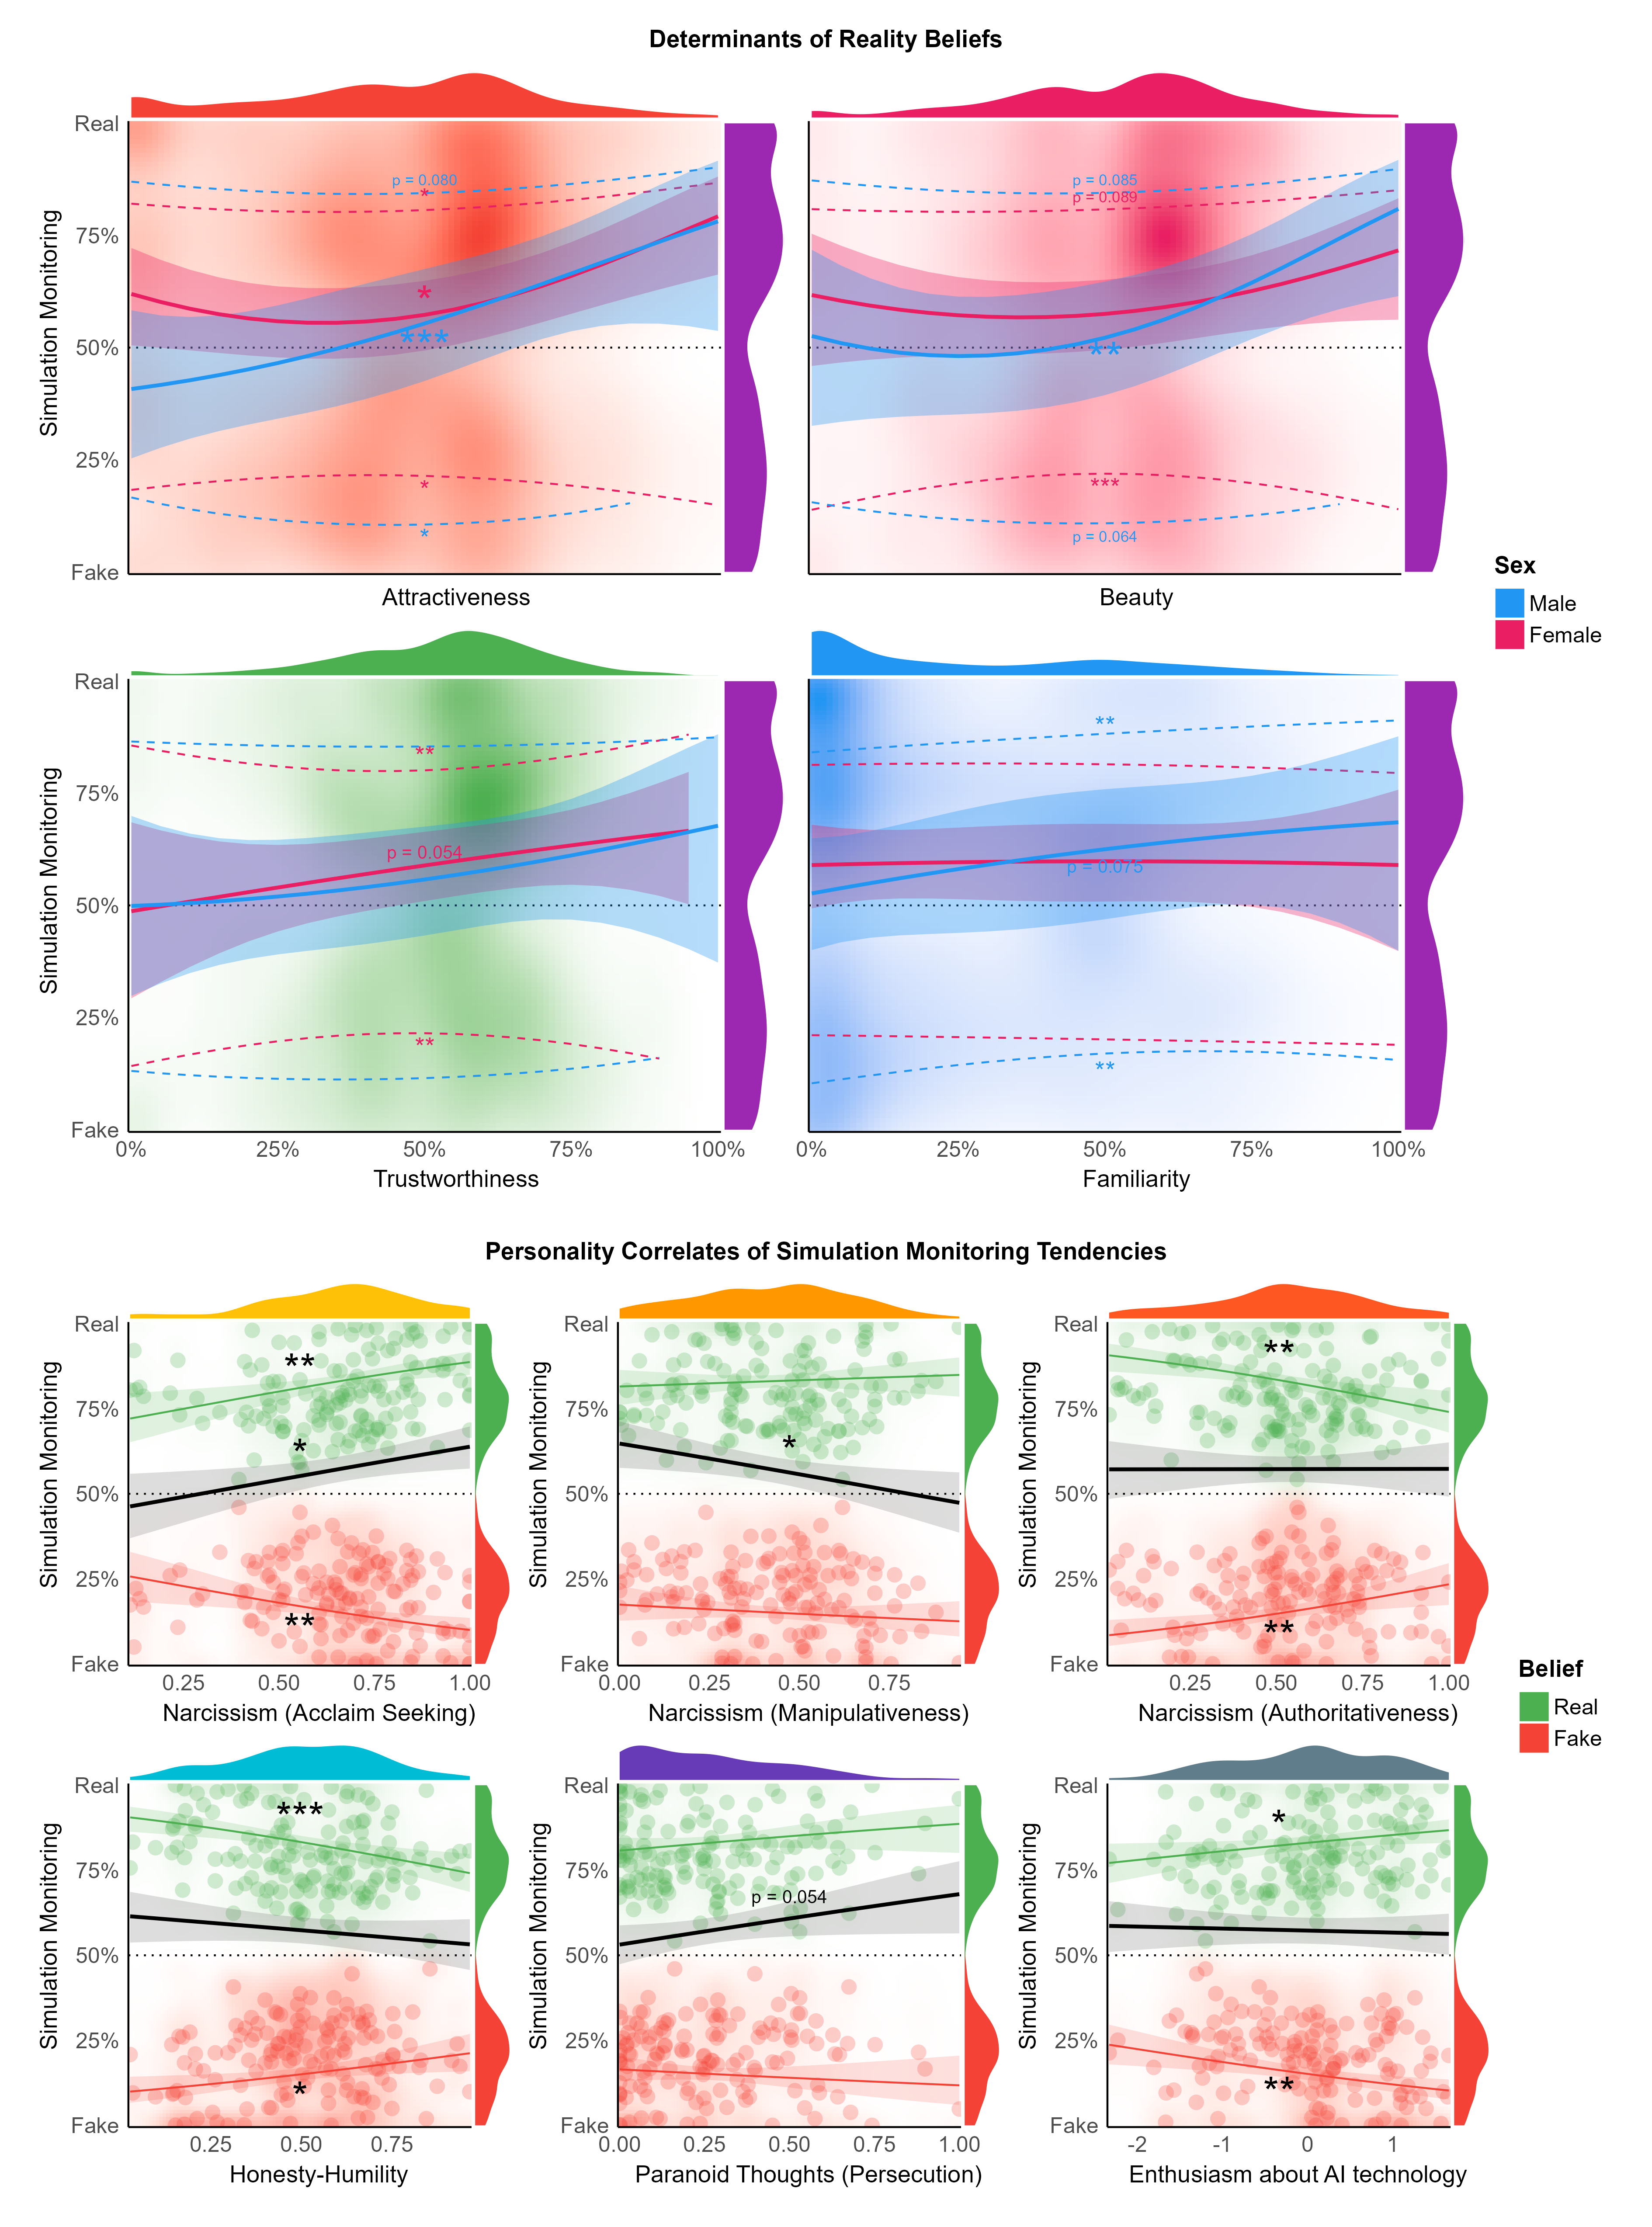
\includegraphics[width=1\linewidth]{../figures/Figure2} \caption{Top part shows blabla.}\label{fig:unnamed-chunk-3}
\end{figure}

Finally, we investigated the inter-individual correlates of simulation monitoring by computing, for each participant, the proportion of faces judged as real (i.e., the overall bias towards one or the other belief), as well as the average confidence for faces judged as real, and fake. We assessed the link between these scores and dispositional traits using Bayesian correlation analysis (Makowski et al., 2020; Makowski, Ben-Shachar, Chen, et al., 2019).

The analysis was carried out using \emph{R 4.2} (R Core Team, 2022), the \emph{tidyverse} (Wickham et al., 2019), and the \emph{easystats} collection of packages (Lüdecke et al., 2021, 2019, 2020; Makowski, Ben-Shachar, \& Lüdecke, 2019). As all the details, scripts and complimentary analyses are open-access, the manuscript will focus on significant results.

\hypertarget{results}{%
\subsection{Results}\label{results}}

\hypertarget{manipulation-check}{%
\subsubsection{Manipulation Check}\label{manipulation-check}}

Only one image file yielded a strong simulation monitoring bias (\textgreater{} 85\%), being classified as fake in 87.4\% of trials. This image was removed from further analysis, leaving 108 trials per participant. On average, across participants, 44\% of images (95\% CI {[}0.11, 0.64{]}) were judged as fake and 56\% of images (95\% CI {[}0.36, 0.89{]}) as real. An intercept-only model with the participants and images as random factors showed that the Intraclass Correlation Coefficient (ICC), which can be interpreted as the proportion of variance explained by the random factors, was of 10.5\% for the participants and 8.7\% for the pictures.

There was a significant negative effect of the delay of re-exposure (with 95\% of values between 1.58 and 30.31 min), suggesting that shorter delays were associated with a slight bias towards the belief of reality (60\% at a theoretical delay of 0), which decreased to 50\% at a theoretical delay of 60 min (\(OR = 0.99\), \(95\% CI = [0.99, 1.00]\), \(z = -2.27\), \(p = .023\)). There was also a significant negative effect on judgment confidence, but only in the real condition (\(\beta = -0.005\), \(95\% CI = [-0.1, 0.0]\), \(p = .023\)).

\hypertarget{determinants-of-simulation-monitoring}{%
\subsubsection{Determinants of Simulation Monitoring}\label{determinants-of-simulation-monitoring}}

Attractiveness had a significant positive and linear relationship (\(R^2_{marginal}\) = 2.8\%) with the belief that a stimulus was real (\(\beta_{poly1} = 16.37\), \(95\% CI = [7.76, 24.98]\), \(z = 3.73\), \(p < .001\)) for males, and a quadratic relationship for females (\(\beta_{poly2} = 7.77\), \(95\% CI = [1.41, 14.13]\), \(z = 2.40\), \(p = .017\)), with both non-attractive and attractive faces being judged as more real. No significant relationship was found between attractiveness ratings and belief confidence, aside of a similar trend for females only, for faces judged as real (\(\beta_{poly2} = 4.38\), \(95\% CI = [0.96, 7.79]\), \(z = 2.51\), \(p = .012\)). There was no interaction with reported self-attractiveness.

Beauty, adjusted for trustworthiness and familiarity, had a significant positive and linear relationship (\(R^2_{marginal}\) = 3.5\%) with the belief that a stimulus was real (\(\beta_{poly1} = 9.54\), \(95\% CI = [1.43, 17.65]\), \(z = 2.31\), \(p = .021\)) for males only. No effect on confidence was found, aside from a quadratic relationship for females for faces judged as fake, suggesting that non-beautiful and highly beautiful faces were rated as fake with more confidence than average faces (\(\beta_{poly2} = 6.61\), \(95\% CI = [1.98, 11.24]\), \(z = 2.80\), \(p = .005\)). There was no interaction with reported self-attractiveness.

Trustworthiness, adjusted for beauty and familiarity, had a significant positive and linear relationship (\(R^2_{marginal}\) = 3.0\%) with the belief that a stimulus was real (\(\beta_{poly1} = 11.60\), \(95\% CI = [4.15, 19.06]\), \(z = 3.05\), \(p = .002\)) for females only. No effect on confidence was found, aside from a quadratic relationship for females for faces judged as real, suggesting that non-trustworthy and highly trustworthy faces were rated as real with more confidence than average faces (\(\beta_{poly2} = 6.47\), \(95\% CI = [1.73, 11.21]\), \(z = 2.68\), \(p = .007\)).

We did not find any significant relationships for familiarity adjusted for beauty and trustworthiness (\(R^2_{marginal}\) = 3.0\%). However, a significant positive and linear relationship was found with the confidence in faces judged as real (\(\beta_{poly1} = 9.31\), \(95\% CI = [3.45, 15.17]\), \(z = -3.11\), \(p = .002\)), and a quadratic relationship for faces judged as fake (\(\beta_{poly1} = -12.67\), \(95\% CI = [-19.87, -5.47]\), \(z = -3.45\), \(p < .001\); \(\beta_{poly2} = 8.14\), \(95\% CI = [0.01, 16.28]\), \(z = 1.96\), \(p = .05\)), for males only, suggesting that faces are judged as real with more confidence when they are familiar, and judged as fake with less confidence when they are of not familiar or highly familiar.

\hypertarget{inter-individual-correlates-of-simulation-monitoring}{%
\subsubsection{Inter-Individual Correlates of Simulation Monitoring}\label{inter-individual-correlates-of-simulation-monitoring}}

Bayesian correlations with personality traits suggested that Honesty-Humility was negatively associated with the confidence in reality (\(r = -0.21\), \(95\% CI = [-0.38, -0.03]\), \(BF_{10} = 3.57\)), and positively associated with the Narcissism trait of Acclaim Seeking (\(r = 0.26\), \(95\% CI = [0.08, 0.43]\), \(BF_{10} = 14.38\)) and Grandiose Fantasies (\(r = 0.22\), \(95\% CI = [0.04, 0.40]\), \(BF_{10} = 4.18\)). Acclaim Seeking was also positively related with the confidence in fake judgments (\(r = 0.22\), \(95\% CI = [0.04, 0.40]\), \(BF_{10} = 4.52\)). No significant correlations was found for social anxiety, intolerance to uncertainty, or paranoid beliefs.

Questions pertaining to the attitude towards AI were reduced to 3 dimensions through factor analysis, labelled AI-Enthusiasm (loaded by items expressing interest and excitement in AI development and applications), AI-Realness (loaded by items expressing positive opinions on the ability of AI to create realistic material), and AI-Danger (loaded by items expressing concerns on the unethical misuse of AI technology). Only AI-Enthusiasm displayed a significant positive relationship with the confidence in both real (\(r = 0.24\), \(95\% CI = [0.06, 0.41]\), \(BF_{10} = 8.00\)) and fake (\(r = 0.28\), \(95\% CI = [0.11, 0.44]\), \(BF_{10} = 23.04\)) judgments.

\hypertarget{discussion}{%
\subsection{Discussion}\label{discussion}}

This study aimed at investigating the effect of facial ratings (attractiveness, beauty, trustworthiness and familiarity) on simulation monitoring, i.e., on the belief that the stimulus is artificially generated. The most striking result, in our opinion, is that despite all the stimuli being real faces from the same database, all participants, when given the information, believed (to high degrees of confidence) that a significant proportion of them were fake. This finding is a testimony to both the current expectations regarding CGI technology in the population, as well as to the volatility of our sense of reality. It underlines the strong impact of prior expectations and information on reality beliefs. In fact, stimuli-related and participant-related characteristics accounted for less than 20\% of the beliefs variance, suggesting that a large part of it is associated with other subjective processes.

Although attractiveness did not seem to be the primary drive underlying simulation monitoring of face images, we do nonetheless report significant associations, with a different pattern depending on the participant's gender. The quadratic relationship found for female participants is aligned with our hypothesis that salient faces (i.e., rated as very attractive or very unattractive) are judged to be more real. Alternatively, we could interpret the mostly positive linear relationship for males under an evolutionary lens. In particular, males purportedly place more emphasis on facial attractiveness as a sign of reproductive potential, as compared with females, who tend to value characteristics signaling resource acquisition capabilities (Fink et al., 2006; Qi \& Ying, 2022). As such, it is possible that the evolutionary weight associated with attractiveness skewed the perceived saliency towards attractive faces, rendering attractive faces are significantly more salient than unattractive ones, in turn distorting the relationship with simulation monitoring. Future studies should test this saliency-based hypothesis by measuring constructs closer to salience and its effects, for instance using neuroimaging (\textbf{ref on saliency in EEG or fMRI}) or physiological markers {[}in particular, heart rate deceleration, \textbf{include refs}{]}.

discuss why the link with beauty is slightly different. Note that for models for beauty we adjusted the models for trustowrthiness and familiarity, hence possibly masking the multidimensionality of attractiveness.

In contrast to the findings for attractiveness, trustworthiness linearly increased beliefs in realness for females only. Given the evidence for the effect in the opposite direction, suggesting that faces presented as were rated as more trustworthy (Balas \& Pacella, 2017; Hoogers, 2021; Liefooghe et al., 2022), we expected such link to be present for both genders. One of the contributing mechanism to this dimorphism could have been the increased risk-taking aversion reported in females (explained evolutionary as a compromise their reproductive potential, Van Den Akker et al., 2020), to which perceived facial trustworthiness relates (Hou \& Liu, 2019). However, faces judged as highly untrustworthy should have appear as even more salient (representing an evolutionary threat), and hence be judged as more real. As such, further studies are needed to investigate the causes of the increased simulation monitoring sensitivity to trustworthiness in females.

Contrary to our hypothesis, familiarity was not found to be significantly related to simulation monitoring decisions. It is to note that the distribution of familiarity ratings was strongly skewed, and that a low number of pictures was rated as highly familiar. Future studies could re-examine this aspect by experimentally manipulating familiarity, for instance by modulating the amount of exposures of items before the simulation monitoring ratings.

Although the order of presentation of the facial images was randomized to reduce effects of adaptation, re-exposure delay was found to have a significant negative effect on simulation monitoring decisions, with shorter delays being associated with faces being rated as more real. Interestingly, while it could be posited that shorter delays led to the faces appearing more familiar and thereby increased people's belief in its realness, this seems unlikely considering perceived familiarity did not significantly affect simulation monitoring decisions made, even after controlling for attractiveness and trustworthiness. Alternatively, shorter re-exposure delays could have led to the faces being better remembered, thus triggering autobiographical memory processes (Gobbini et al., 2013) and evoking a sense of personal relevance during the repeated display. Indeed, fictional stimuli that were associated with more personal memories have been shown to up-regulate emotions (Makowski et al., 2017; Sperduti et al., 2016), thus biasing the realness of the given stimulus

\hypertarget{acknowledgments}{%
\section{Acknowledgments}\label{acknowledgments}}

We would like to thank \textbf{TODO: add STUDENT NAME} for his contribution to the selection of the materials.

\newpage

\hypertarget{references}{%
\section{References}\label{references}}

\hypertarget{refs}{}
\begin{CSLReferences}{1}{0}
\leavevmode\vadjust pre{\hypertarget{ref-bago2022emotion}{}}%
Bago, B., Rosenzweig, L. R., Berinsky, A. J., \& Rand, D. G. (2022). Emotion may predict susceptibility to fake news but emotion regulation does not seem to help. \emph{Cognition and Emotion}, 1--15.

\leavevmode\vadjust pre{\hypertarget{ref-balas2017}{}}%
Balas, B., \& Pacella, J. (2017). Trustworthiness perception is disrupted in artificial faces. \emph{Computers in Human Behavior}, \emph{77}. \url{https://doi.org/10.1016/j.chb.2017.08.045}

\leavevmode\vadjust pre{\hypertarget{ref-bartosik2021you}{}}%
Bartosik, B., Wojcik, G. M., Brzezicka, A., \& Kawiak, A. (2021). Are you able to trust me? Analysis of the relationships between personality traits and the assessment of attractiveness and trust. \emph{Frontiers in Human Neuroscience}, \emph{15}, 685530.

\leavevmode\vadjust pre{\hypertarget{ref-begg1992dissociation}{}}%
Begg, I. M., Anas, A., \& Farinacci, S. (1992). Dissociation of processes in belief: Source recollection, statement familiarity, and the illusion of truth. \emph{Journal of Experimental Psychology: General}, \emph{121}(4), 446.

\leavevmode\vadjust pre{\hypertarget{ref-berghel2018weaponizing}{}}%
Berghel, H. (2018). Weaponizing twitter litter: Abuse-forming networks and social media. \emph{Computer}, \emph{51}(4), 70--73.

\leavevmode\vadjust pre{\hypertarget{ref-britt2019reasoned}{}}%
Britt, M. A., Rouet, J.-F., Blaum, D., \& Millis, K. (2019). A reasoned approach to dealing with fake news. \emph{Policy Insights from the Behavioral and Brain Sciences}, \emph{6}(1), 94--101.

\leavevmode\vadjust pre{\hypertarget{ref-bryanov2021determinants}{}}%
Bryanov, K., \& Vziatysheva, V. (2021). Determinants of individuals' belief in fake news: A scoping review determinants of belief in fake news. \emph{PLoS One}, \emph{16}(6), e0253717.

\leavevmode\vadjust pre{\hypertarget{ref-calbi2017}{}}%
Calbi, M., Heimann, K., Barratt, D., Siri, F., Umiltà, M. A., \& Gallese, V. (2017). How context influences our perception of emotional faces: A behavioral study on the kuleshov effect. \emph{Frontiers in Psychology}, \emph{8}. \url{https://www.frontiersin.org/articles/10.3389/fpsyg.2017.01684}

\leavevmode\vadjust pre{\hypertarget{ref-carleton2007fearing}{}}%
Carleton, R. N., Norton, M. P. J., \& Asmundson, G. J. (2007). Fearing the unknown: A short version of the intolerance of uncertainty scale. \emph{Journal of Anxiety Disorders}, \emph{21}(1), 105--117.

\leavevmode\vadjust pre{\hypertarget{ref-chen2021broadening}{}}%
Chen, J. M., Norman, J. B., \& Nam, Y. (2021). Broadening the stimulus set: Introducing the american multiracial faces database. \emph{Behavior Research Methods}, \emph{53}(1), 371--389.

\leavevmode\vadjust pre{\hypertarget{ref-chen2015news}{}}%
Chen, Y., Conroy, N. K., \& Rubin, V. L. (2015). News in an online world: The need for an {``automatic crap detector.''} \emph{Proceedings of the Association for Information Science and Technology}, \emph{52}(1), 1--4.

\leavevmode\vadjust pre{\hypertarget{ref-de2015jspsych}{}}%
De Leeuw, J. R. (2015). jsPsych: A JavaScript library for creating behavioral experiments in a web browser. \emph{Behavior Research Methods}, \emph{47}(1), 1--12.

\leavevmode\vadjust pre{\hypertarget{ref-ecker2022psychological}{}}%
Ecker, U. K., Lewandowsky, S., Cook, J., Schmid, P., Fazio, L. K., Brashier, N., Kendeou, P., Vraga, E. K., \& Amazeen, M. A. (2022). The psychological drivers of misinformation belief and its resistance to correction. \emph{Nature Reviews Psychology}, \emph{1}(1), 13--29.

\leavevmode\vadjust pre{\hypertarget{ref-fink2006facial}{}}%
Fink, B., Neave, N., Manning, J. T., \& Grammer, K. (2006). Facial symmetry and judgements of attractiveness, health and personality. \emph{Personality and Individual Differences}, \emph{41}(3), 491--499.

\leavevmode\vadjust pre{\hypertarget{ref-freeman2021revised}{}}%
Freeman, D., Loe, B. S., Kingdon, D., Startup, H., Molodynski, A., Rosebrock, L., Brown, P., Sheaves, B., Waite, F., \& Bird, J. C. (2021). The revised green et al., Paranoid thoughts scale (r-GPTS): Psychometric properties, severity ranges, and clinical cut-offs. \emph{Psychological Medicine}, \emph{51}(2), 244--253.

\leavevmode\vadjust pre{\hypertarget{ref-garrido2017kdef}{}}%
Garrido, M. V., \& Prada, M. (2017). KDEF-PT: Valence, emotional intensity, familiarity and attractiveness ratings of angry, neutral, and happy faces. \emph{Frontiers in Psychology}, \emph{8}, 2181.

\leavevmode\vadjust pre{\hypertarget{ref-gobbini2013prioritized}{}}%
Gobbini, M. I., Gors, J. D., Halchenko, Y. O., Rogers, C., Guntupalli, J. S., Hughes, H., \& Cipolli, C. (2013). Prioritized detection of personally familiar faces. \emph{PloS One}, \emph{8}(6), e66620.

\leavevmode\vadjust pre{\hypertarget{ref-goldstein2009pleasure}{}}%
Goldstein, T. R. (2009). The pleasure of unadulterated sadness: Experiencing sorrow in fiction, nonfiction, and" in person.". \emph{Psychology of Aesthetics, Creativity, and the Arts}, \emph{3}(4), 232.

\leavevmode\vadjust pre{\hypertarget{ref-hoogers2021effect}{}}%
Hoogers, E. (2021). \emph{The effect of attitude towards computer generated faces on face perception} {[}\{B.S.\} thesis{]}.

\leavevmode\vadjust pre{\hypertarget{ref-hou2019survival}{}}%
Hou, C., \& Liu, Z. (2019). The survival processing advantage of face: The memorization of the (un) trustworthy face contributes more to survival adaptation. \emph{Evolutionary Psychology}, \emph{17}(2), 1474704919839726.

\leavevmode\vadjust pre{\hypertarget{ref-jauk2022validation}{}}%
Jauk, E., Olaru, G., Schürch, E., Back, M. D., \& Morf, C. C. (2022). Validation of the german five-factor narcissism inventory and construction of a brief form using ant colony optimization. \emph{Assessment}, 10731911221075761.

\leavevmode\vadjust pre{\hypertarget{ref-lewandowsky2017beyond}{}}%
Lewandowsky, S., Ecker, U. K., \& Cook, J. (2017). Beyond misinformation: Understanding and coping with the {``post-truth''} era. \emph{Journal of Applied Research in Memory and Cognition}, \emph{6}(4), 353--369.

\leavevmode\vadjust pre{\hypertarget{ref-liefooghe2022faces}{}}%
Liefooghe, B., Oliveira, M., Leisten, L. M., Hoogers, E., Aarts, H., \& Hortensius, R. (2022). \emph{Faces merely labelled as artificial are trusted less}.

\leavevmode\vadjust pre{\hypertarget{ref-little2011facial}{}}%
Little, A. C., Jones, B. C., \& DeBruine, L. M. (2011). Facial attractiveness: Evolutionary based research. \emph{Philosophical Transactions of the Royal Society B: Biological Sciences}, \emph{366}(1571), 1638--1659.

\leavevmode\vadjust pre{\hypertarget{ref-parametersArticle}{}}%
Lüdecke, D., Ben-Shachar, M., Patil, I., \& Makowski, D. (2020). Extracting, computing and exploring the parameters of statistical models using {R}. \emph{Journal of Open Source Software}, \emph{5}(53), 2445. \url{https://doi.org/10.21105/joss.02445}

\leavevmode\vadjust pre{\hypertarget{ref-performanceArticle}{}}%
Lüdecke, D., Ben-Shachar, M., Patil, I., Waggoner, P., \& Makowski, D. (2021). {performance}: An {R} package for assessment, comparison and testing of statistical models. \emph{Journal of Open Source Software}, \emph{6}(60), 3139. \url{https://doi.org/10.21105/joss.03139}

\leavevmode\vadjust pre{\hypertarget{ref-insightArticle}{}}%
Lüdecke, D., Waggoner, P., \& Makowski, D. (2019). Insight: A unified interface to access information from model objects in {R}. \emph{Journal of Open Source Software}, \emph{4}(38), 1412. \url{https://doi.org/10.21105/joss.01412}

\leavevmode\vadjust pre{\hypertarget{ref-makowski2018cognitive}{}}%
Makowski, D. (2018). \emph{Cognitive neuropsychology of implicit emotion regulation through fictional reappraisal} {[}PhD thesis{]}. Sorbonne Paris Cit{é}.

\leavevmode\vadjust pre{\hypertarget{ref-makowski2019indices}{}}%
Makowski, D., Ben-Shachar, M. S., Chen, S. A., \& Lüdecke, D. (2019). Indices of effect existence and significance in the bayesian framework. \emph{Frontiers in Psychology}, \emph{10}, 2767.

\leavevmode\vadjust pre{\hypertarget{ref-bayestestRArticle}{}}%
Makowski, D., Ben-Shachar, M., \& Lüdecke, D. (2019). {bayestestR}: Describing effects and their uncertainty, existence and significance within the {Bayesian} framework. \emph{Journal of Open Source Software}, \emph{4}(40), 1541. \url{https://doi.org/10.21105/joss.01541}

\leavevmode\vadjust pre{\hypertarget{ref-correlationArticle}{}}%
Makowski, D., Ben-Shachar, M., Patil, I., \& Lüdecke, D. (2020). Methods and algorithms for correlation analysis in {R}. \emph{Journal of Open Source Software}, \emph{5}(51), 2306. \url{https://doi.org/10.21105/joss.02306}

\leavevmode\vadjust pre{\hypertarget{ref-makowski2017being}{}}%
Makowski, D., Sperduti, M., Nicolas, S., \& Piolino, P. (2017). {``Being there''} and remembering it: Presence improves memory encoding. \emph{Consciousness and Cognition}, \emph{53}, 194--202.

\leavevmode\vadjust pre{\hypertarget{ref-makowski2019phenomenal}{}}%
Makowski, D., Sperduti, M., Pelletier, J., Blondé, P., La Corte, V., Arcangeli, M., Zalla, T., Lemaire, S., Dokic, J., Nicolas, S., et al. (2019). Phenomenal, bodily and brain correlates of fictional reappraisal as an implicit emotion regulation strategy. \emph{Cognitive, Affective, \& Behavioral Neuroscience}, \emph{19}(4), 877--897.

\leavevmode\vadjust pre{\hypertarget{ref-martel2020reliance}{}}%
Martel, C., Pennycook, G., \& Rand, D. G. (2020). Reliance on emotion promotes belief in fake news. \emph{Cognitive Research: Principles and Implications}, \emph{5}(1), 1--20.

\leavevmode\vadjust pre{\hypertarget{ref-mcdonnell2010face}{}}%
McDonnell, R., \& Breidt, M. (2010). Face reality: Investigating the uncanny valley for virtual faces. In \emph{ACM SIGGRAPH ASIA 2010 sketches} (pp. 1--2).

\leavevmode\vadjust pre{\hypertarget{ref-michael2021source}{}}%
Michael, R. B., \& Sanson, M. (2021). Source information affects interpretations of the news across multiple age groups in the united states. \emph{Societies}, \emph{11}(4), 119.

\leavevmode\vadjust pre{\hypertarget{ref-moshel2022}{}}%
Moshel, M. L., Robinson, A. K., Carlson, T. A., \& Grootswagers, T. (2022). Are you for real? Decoding realistic AI-generated faces from neural activity. \emph{Vision Research}, \emph{199}, 108079. \url{https://doi.org/10.1016/j.visres.2022.108079}

\leavevmode\vadjust pre{\hypertarget{ref-nightingale2022}{}}%
Nightingale, S. J., \& Farid, H. (2022). AI-synthesized faces are indistinguishable from real faces and more trustworthy. \emph{Proceedings of the National Academy of Sciences}, \emph{119}(8), e2120481119. \url{https://doi.org/10.1073/pnas.2120481119}

\leavevmode\vadjust pre{\hypertarget{ref-pantserev2020}{}}%
Pantserev, K. (2020). \emph{The malicious use of AI-based deepfake technology as the new threat to psychological security and political stability} (pp. 37--55). \url{https://doi.org/10.1007/978-3-030-35746-7_3}

\leavevmode\vadjust pre{\hypertarget{ref-peer2022}{}}%
Peer, E., Rothschild, D., Gordon, A., Evernden, Z., \& Damer, E. (2022). Data quality of platforms and panels for online behavioral research. \emph{Behavior Research Methods}, \emph{54}(4), 1643--1662. \url{https://doi.org/10.3758/s13428-021-01694-3}

\leavevmode\vadjust pre{\hypertarget{ref-pehlivanoglu2021role}{}}%
Pehlivanoglu, D., Lin, T., Deceus, F., Heemskerk, A., Ebner, N. C., \& Cahill, B. S. (2021). The role of analytical reasoning and source credibility on the evaluation of real and fake full-length news articles. \emph{Cognitive Research: Principles and Implications}, \emph{6}(1), 1--12.

\leavevmode\vadjust pre{\hypertarget{ref-pennycook2019lazy}{}}%
Pennycook, G., \& Rand, D. G. (2019). Lazy, not biased: Susceptibility to partisan fake news is better explained by lack of reasoning than by motivated reasoning. \emph{Cognition}, \emph{188}, 39--50.

\leavevmode\vadjust pre{\hypertarget{ref-peters2012development}{}}%
Peters, L., Sunderland, M., Andrews, G., Rapee, R. M., \& Mattick, R. P. (2012). Development of a short form social interaction anxiety (SIAS) and social phobia scale (SPS) using nonparametric item response theory: The SIAS-6 and the SPS-6. \emph{Psychological Assessment}, \emph{24}(1), 66.

\leavevmode\vadjust pre{\hypertarget{ref-petty1986elaboration}{}}%
Petty, R. E., \& Cacioppo, J. T. (1986). The elaboration likelihood model of persuasion. In \emph{Communication and persuasion} (pp. 1--24). Springer.

\leavevmode\vadjust pre{\hypertarget{ref-piksa2022cognitive}{}}%
Piksa, M., Noworyta, K., Piasecki, J., Gwiazdzinski, P., Gundersen, A. B., Kunst, J., \& Rygula, R. (2022). Cognitive processes and personality traits underlying four phenotypes of susceptibility to (mis) information. \emph{Frontiers in Psychiatry}, 1142.

\leavevmode\vadjust pre{\hypertarget{ref-qi2022gender}{}}%
Qi, Y., \& Ying, J. (2022). Gender biases in the accuracy of facial judgments: Facial attractiveness and perceived socioeconomic status. \emph{Frontiers in Psychology}, \emph{13}.

\leavevmode\vadjust pre{\hypertarget{ref-RCoreTeam2022}{}}%
R Core Team. (2022). \emph{R: A language and environment for statistical computing}. R Foundation for Statistical Computing. \url{https://www.R-project.org/}

\leavevmode\vadjust pre{\hypertarget{ref-sanchez2005presence}{}}%
Sanchez-Vives, M. V., \& Slater, M. (2005). From presence to consciousness through virtual reality. \emph{Nature Reviews Neuroscience}, \emph{6}(4), 332--339.

\leavevmode\vadjust pre{\hypertarget{ref-schepman2020initial}{}}%
Schepman, A., \& Rodway, P. (2020). Initial validation of the general attitudes towards artificial intelligence scale. \emph{Computers in Human Behavior Reports}, \emph{1}, 100014.

\leavevmode\vadjust pre{\hypertarget{ref-sibley2011}{}}%
Sibley, C., Luyten, N., Wolfman, M., Mobberley, A., Wootton, L. W., Hammond, M., Sengupta, N., Perry, R., West-Newman, T., Wilson, M., McLellan, L., Hoverd, W. J., \& Robertson, A. (2011). The mini-IPIP6: Validation and extension of a short measure of the big-six factors of personality in new zealand. \emph{New Zealand Journal of Psychology}, \emph{40}, 142--159.

\leavevmode\vadjust pre{\hypertarget{ref-sindermann2020short}{}}%
Sindermann, C., Cooper, A., \& Montag, C. (2020). A short review on susceptibility to falling for fake political news. \emph{Current Opinion in Psychology}, \emph{36}, 44--48.

\leavevmode\vadjust pre{\hypertarget{ref-sobieraj2014beautiful}{}}%
Sobieraj, S., \& Krämer, N. C. (2014). What is beautiful in cyberspace? Communication with attractive avatars. \emph{International Conference on Social Computing and Social Media}, 125--136.

\leavevmode\vadjust pre{\hypertarget{ref-sperduti2016paradox}{}}%
Sperduti, M., Arcangeli, M., Makowski, D., Wantzen, P., Zalla, T., Lemaire, S., Dokic, J., Pelletier, J., \& Piolino, P. (2016). The paradox of fiction: Emotional response toward fiction and the modulatory role of self-relevance. \emph{Acta Psychologica}, \emph{165}, 53--59.

\leavevmode\vadjust pre{\hypertarget{ref-sperduti2017distinctive}{}}%
Sperduti, M., Makowski, D., Arcangeli, M., Wantzen, P., Zalla, T., Lemaire, S., Dokic, J., Pelletier, J., \& Piolino, P. (2017). The distinctive role of executive functions in implicit emotion regulation. \emph{Acta Psychologica}, \emph{173}, 13--20.

\leavevmode\vadjust pre{\hypertarget{ref-susmann2021persuasion}{}}%
Susmann, M. W., Xu, M., Clark, J. K., Wallace, L. E., Blankenship, K. L., Philipp-Muller, A. Z., Luttrell, A., Wegener, D. T., \& Petty, R. E. (2021). Persuasion amidst a pandemic: Insights from the elaboration likelihood model. \emph{European Review of Social Psychology}, 1--37.

\leavevmode\vadjust pre{\hypertarget{ref-tsikandilakis2019beauty}{}}%
Tsikandilakis, M., Bali, P., \& Chapman, P. (2019). Beauty is in the eye of the beholder: The appraisal of facial attractiveness and its relation to conscious awareness. \emph{Perception}, \emph{48}(1), 72--92.

\leavevmode\vadjust pre{\hypertarget{ref-tucciarelli2020}{}}%
Tucciarelli, R., Vehar, N., \& Tsakiris, M. (2020). \emph{On the realness of people who do not exist: the social processing of artificial faces}. \url{https://doi.org/10.31234/osf.io/dnk9x}

\leavevmode\vadjust pre{\hypertarget{ref-van2020sex}{}}%
Van Den Akker, O. R., Assen, M. A. van, Van Vugt, M., \& Wicherts, J. M. (2020). Sex differences in trust and trustworthiness: A meta-analysis of the trust game and the gift-exchange game. \emph{Journal of Economic Psychology}, \emph{81}, 102329.

\leavevmode\vadjust pre{\hypertarget{ref-wickham2019}{}}%
Wickham, H., Averick, M., Bryan, J., Chang, W., McGowan, L. D., François, R., Grolemund, G., Hayes, A., Henry, L., Hester, J., Kuhn, M., Pedersen, T. L., Miller, E., Bache, S. M., Müller, K., Ooms, J., Robinson, D., Seidel, D. P., Spinu, V., \ldots{} Yutani, H. (2019). Welcome to the {tidyverse}. \emph{Journal of Open Source Software}, \emph{4}(43), 1686. \url{https://doi.org/10.21105/joss.01686}

\end{CSLReferences}


\clearpage
\renewcommand{\listfigurename}{Figure captions}


\end{document}
